

% Some notes on what is left to do
%
%  Chapter introduction 
%  Branching processes section 
%  Check and tidy QS stuff
%  Check and tidy survivor stuff
%  Check and tidy MOC stuff
%  Add simple BD derivation to the MOC section
%
%
%
%


























%%%%%%%%%%%%%%%%%%%%%%%%%%%%%%%%%%%%%%%%%%%%%%%%%%%%%%%%%%%%%%%%%%%%% Branching processes 




















\chapter{Mathematical background}


\begin{itemize}
\item In the case of slightly supercritical branching,  the initial count of replicative individuals weighs heavily on the chance of overall process survival.

\item In the case of subcritical branching,  when conditioning on process non-death, the expected individual count tends to a constant (a quasi-stationary mean).  The value of this, $\mean{\xt| \xt>0}$, grows to infinity in the limit of the process becoming critical from below.  In the case of the continuous time birth-death process, we can describe the inverse of this conditional mean with a formula; in the case of the discrete Galton-Watson process,  we tried to find the (yet unknown) equivalent formula.  Despite ultimately not finding it, we still think it is attainable.  
\end{itemize}





%%%%%%%%%%%%%%%%%%%%%%%%%%%%%%%%%%%%%%%%%%%%%%%%%%%%%%%%%%%%%%%%%%%%%%%%%%%%%%%%%%%%%%%%%%%%%%%%% Special 1 criticallity thing




\section{Limiting conditional distribution}



Suppose each individual produces, at the end of its life, independently, a number of offspring that is a random variable $\xx$, with 
$$\pr{\xx = k} = p_k, \hspace{20pt} k = 0,1,2,\dots$$
Denote the mean number of offspring per individual by 
$$\mu=\mean{\xx}$$
Let ${\bf Z}_n$ be the number of individuals in the $n$th generation. Then $\mean{\zz_n|\zz_0=1} = \mu^n.$ If $\mu < 1$ then $\lim_{n\to \infty}{\pr{\zz_n = 0}} = 1$. The population is guaranteed to go extinct.

Denote the probability generating function of $\xx$ as 
$$\phi(z) = \mean{z^{\xx}},$$
and the probability of population extinction by generation $n$ as 
$\pr{\zz_n = 0} = u_n.$
Then, as can be seen from a first step argument, it holds that 
\begin{equation}
\label{iterPGF}
u_{n+1} = \phi(u_n).
\end{equation}

\subsection{Death or division}
Consider the specific case: 
\begin{align*}
p_2 &= P &&\text{(division)}  \\
p_0 &= 1-P && \text{(death)}\\
p_i &= 0 \hspace{20pt} \forall i \neq 0,2  
\end{align*}

\noindent
In this case the mean number of offspring per individual takes the value,
$$\mu = 2P.$$
And so the expected population size resulting from a single offspring will be
$$\mean{\zz_n} = (2P)^n.$$
From (\ref{iterPGF}), we see
\begin{equation}
\label{unIter}
u_{n+1} = 1-P + P u_n^2.
\end{equation}
With $u_n$ the probability of extinction, let us also denote its complement
$$S_n = 1-u_n,$$
the probability of population persistence at generation $n$. 

From (\ref{unIter}), it can be shown that
\begin{equation}
\label{SnIter}
S_{n+1} = 2P S_n - PS_n^2.
\end{equation}

\subsection{Late time persistence probability, $S_n$}

Considering the case where $P < 0.5$, in which death of an individual is more probable than its reproduction, the expected population size will tend towards 0 with increasing $n$; the probability of non-extinction too will approach 0. 

As it does so, $S_n^2$ becomes insignificant in comparison to $S_n$. For this reason, the iterative relation, (\ref{SnIter}), will increasingly satisfy
\begin{equation}
\label{attenuated}
S_{n+1} \approx 2PS_n.
\end{equation}
So at late time ($n\to\infty$), it will be found that
\begin{equation}
\label{lateS}
S_n \sim A\,(2P)^n\qquad (n\to\infty),\quad A=\lim_{m\to\infty}S_m/(2P)^m.
\end{equation}
(The limit of $S_n$ itself is $0$ for $P<\tfrac12$; one must not write $\lim S_n = A(2P)^n$ as an ordinary limit identity.)
The multiplying constant, $A$, might be interpreted as those lingering conditions on $S_n$ accumulated before attenuation to (\ref{attenuated}). In any case, it can be demonstrated computationally: 


\begin{figure}[ht]
\centering
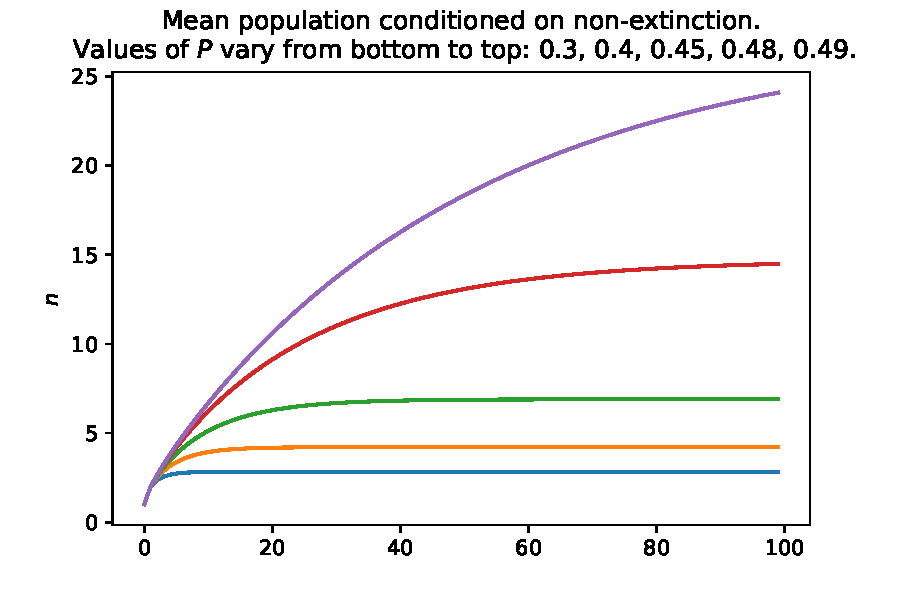
\includegraphics[width = 0.8\textwidth]{chapter3/IMG_ch3/conditionalMean.pdf}
    \label{fig:image}
\end{figure}

\noindent
Figure \ref{fig:image} shows $(2P)^n / S_n$ plotted over successive generations, $n$. In the code, $S_n$ is calculated iteratively using (\ref{SnIter}). The lines were generated with different values of $P$, those at the top closer to the critical state; the purple line was made with $P = 0.49$, the blue at the bottom, $P=0.3$. It is clear that this ratio will tend to a constant value towards large $n$.  

\subsection{Quasi-stationarity}

It is often the case in stochastic processes, as it is in this one for $P<0.5$, that fixation to a particular state is inevitable. Although, in certain cases, it can be observed that before absorption to some final state, behaviour becomes predictable according to some unchanging distribution. This phenomenon has been termed quasi-stationarity. 


\subsection{Mean}
Such behaviour can be observed in a population evolving by the update rules stated above. For demonstration, consider the mean number of individuals from a single ancestor, conditioned on non-extinction: 
$$\mean{\xx_n} = \pr{\xx_n =0} \cancelto{0}{\mean{\xx_n|\xx_n =0}}  + \pr{\xx_n \neq 0}\mean{\xx_n|\xx_n \neq0}.$$
It follows that 
$$\mean{\xx_n|\xx_n \neq 0} =\frac{\mean{\xx_n}}{\pr{\xx_n\neq 0}} = \frac{(2P)^n}{S_n} .$$ 
Then, due to (\ref{lateS}), as $n\to\infty$
$$\mean{\xx_n|\xx_n \neq 0} \to \frac{(2P)^n}{A(2P)^n} = \frac{1}{A};$$
At late time, the remaining non-extinct population tends to a constant expected size.

\subsection{Variance}

\subsubsection{Computing the second moment, $\mean{\xx_n^2}$}

For a random variable, $\xx$, the moment generating function is defined, $\mean{\ee^{t\xx}}$. It can also be written in terms of the probability generating function, $\phi(\ee^t)$. For variable, $\xx$ in question, the pgf is 
\begin{equation*}
\phi_1(z) = Pz^2 + (1-P),
\end{equation*}
and the mgf is 
\begin{equation}
\label{mgf1}
M_1(t) = \phi_1(\ee^t) = P\ee^{2t} + (1-P).
\end{equation}
The subscript 1 indicates relevance to generation $n = 1$. Moments are obtained from $M_n(t)$ in the following way.
\begin{equation}
\label{mgf2}
\mean{\xx_n^r} = \frac{\dd^r}{\dd t^r} M_n(t)\bigg|_{t=0}.
\end{equation}
For example, to get the second moment of $\xx_1$, we can differentiate (\ref{mgf1}) twice, and evaluate the result at $t=0$:
$$ \frac{\dd^2}{\dd t^2} M_1(t)\bigg|_{t=0} = 4P\ee^{2t}\big|_{t=0} = 4P.$$
Quantifying the process' second moment is important when it comes to computing the population variance for successive iterations. But this is only the second moment of the first generation size. To obtain its value for any generation $n$, we must dig a little deeper.  

Following (\ref{mgf2}), we seek to differentiate the moment generating function twice. To start with, let us represent the $n$th mgf in terms of probability generating functions. Recall,
$$\phi_n(z) = \underset{n \text{ times}}{\underbrace{ \phi_{1}\hspace{-2pt}\lrb{\phi_1\hspace{-2pt}\lrb{\dots\phi_1\hspace{-2pt}\lrb{z}}}    }}.$$  
So it follows that 
$$M_n(t) = \phi_1\lrbq{\phi_1\lrbq{\dots\phi_1\lrbq{\ee^t}}}.$$
Differentiating this once, 
\begin{equation}
\label{dmgf1}
M_n'(t) = \phi_1'\lrbq{\phi_{n-1}\lrbq{\ee^t}}  \cdot  \phi_1'\lrbq{\phi_{n-2}\lrbq{\ee^t}}  \cdots   \phi_1'\lrbq{\phi_{1}\lrbq{\ee^t}} \cdot \phi_1'\lrbq{\ee^t} \cdot\ee^t.
\end{equation}
Because 
$$\phi_1'\lrbq{\phi_k\lrbq{\ee^t}} = \frac{\dd}{\dd \phi_k\lrbq{\ee^t}}\bigg(P[\phi_k\lrbq{\ee^t}]^2 + (1-P)\bigg) = 2P \phi_k\lrbq{\ee^t},$$
and $\phi_1'\lrbq{\ee^t} = 2P\ee^t$, (\ref{dmgf1}) is equivalent to 
$$M_n'(t) = (2P)\phi_{n-1}\lrbq{\ee^t}  \cdot  (2P)\phi_{n-2}\lrbq{\ee^t} \cdots (2P)\phi_{1}\lrbq{\ee^t} \cdot (2P)\ee^{2t}.$$
Which in turn can be written as
\begin{equation}
\label{dmgf2}
M_n'(t) = (2P)^n \cdot M_{n-1}(t)  \cdot  M_{n-2}(t)  \cdots M_{1}(t)  \cdot \ee^{2t}.
\end{equation}
Before differentiating this a second time, it is instructive to note that each of the multiplied components, when evaluated at $t=0$ become 1; $M_k(0) = 1$ $\forall k$, and $\ee^{2\times 0} = 1$. 

So, when evaluating the second derivative at $t=0$, it will be seen that many of the parts simplify. This is because, with the expression being a combination of multiplied functions of $t$, differentiating by $t$ will result in a sum of terms. Each element of the sum will be like (\ref{dmgf2}), but with one of the components differentiated wrt t. This is just the product rule ---
\begin{align*}
M_n''(t) = (2P)^n\bigg[  &M_{n-1}'(t)  \cdot  M_{n-2}(t)  \cdots M_{1}(t)  \cdot \ee^{2t} \\
+ &M_{n-1}(t)  \cdot  M_{n-2}'(t)  \cdots M_{1}(t)  \cdot \ee^{2t} \\
&\hspace{65pt}\cdots\\
+ &M_{n-1}(t)  \cdot  M_{n-2}(t)  \cdots M_{1}'(t)  \cdot \ee^{2t} \\
+ &M_{n-1}(t)  \cdot  M_{n-2}(t)  \cdots M_{1}(t)  \cdot 2\ee^{2t} \bigg].
\end{align*}
And as most of the components become 1 with $t=0$,
\begin{equation*}
M_n''(0) = (2P)^n\lrbs{M_{n-1}'(0) + M_{n-2}'(0) + \cdots + M_1'(0) + 2}.
\end{equation*}
$M_k'(0)$ is simply the mean population at generation $k$, so
\begin{equation*}
M_n''(0) = (2P)^n\lrbs{(2P)^{n-1} + (2P)^{n-2} + \cdots + (2P) + 2} = (2P)^n\lrbs{\sum^{n-1}_{i = 0}\lrb{(2P)^i} + 1}.
\end{equation*}
Using the finite geometric series sum, $\sum_{i=1}^n r^{i-1} = (1-r^n)/(1-r)$, 
\begin{equation*}
\mean{\xx_n^2} = M_n''(0) = (2P)^n\lrbs{\frac{1-(2P)^n}{1-2P} + 1};
\end{equation*}
rearranging,
\begin{equation}
\label{secondMoment}
\mean{\xx_n^2}  = (2P)^n\lrb{1 + \frac{1}{1-2P}} - (2P)^{2n}\lrb{\frac{1}{1-2P}}.
\end{equation}
(The minus sign is required: at $n=1$ the expression must return $\mean{\xx_1^2}=4P$.)



\subsubsection{Late time variance}
Var($\xx_n$) is computed using $\mean{\xx_n^2} - \mean{\xx_n}^2$. With (\ref{secondMoment}), we can write,
$$\text{Var}(\xx_n) = (2P)^n\lrb{1 + \frac{1}{1-2P}} - (2P)^{2n}\lrb{\frac{1}{1-2P}} - (2P)^{2n}.$$
For $2P < 1$, at large $n$, $(2P)^{2n}$ will become insignificant in comparison to $(2P)^n$. Hence, as $n\to\infty$,
$$\text{Var}(\xx_n) \to (2P)^n\lrb{1 + \frac{1}{1-2P}}.$$
It's tempting to jump straight from this, to a conclusion that the variance conditional on $\xx_n \neq 0 $ is stationary. But let's not get ahead of ourselves and start from the conditional moments:
$$\mean{\xx_n^2|\xx_n\neq 0} = \frac{\mean{\xx_n^2}}{S_n} \xrightarrow{n\to\infty}   \frac{(2P)^n\lrb{1 + \frac{1}{1-2P}}}{A(2P)^n} = A^{-1}\lrb{1 + \frac{1}{1-2P}}$$
$$\mean{\xx_n|\xx_n\neq 0} =  \frac{\mean{\xx_n}}{S_n}  \xrightarrow{n\to\infty}    \frac{(2P)^n}{A(2P)^n} = A^{-1}$$
From this, it can be seen that the conditional variance will indeed tend to a constant value at late time:
\begin{equation*}
\text{Var}(\xx_n|\xx_n\neq0) = \frac{1}{A}\lrb{1+\frac{1}{1-2P}} - \frac{1}{A^2}.
\end{equation*}



\subsection{Quantifying the quasi-stationary distribution}

We are yet to compute the constant $A$, but so far, Grant has shown that (\ref{SnIter}) can be written as 
$$S_{n+1} - S_n = -rS_n - PS_n^2,$$
($r = 1-2P$). Which in the large $n$ limit will satisfy
$$\frac{\dd S(x)}{\dd x} = -(1-2P)S_n = PS^2,$$
a Riccati equation with solution
$$S(x) = \frac{rB}{e^{rx} +- PB},$$
$B$ constant. 




































%%%%%%%%%%%%%%%%%%%%%%%%%%%%%%%%%%%%%%%%%%%%%%%%%%%%%%%%%%%%%%%%%%%%% special 2 small




\section{Survivability of small populations}
Consider the basic Galton Watson process where each cell leaves behind two daughters or dies. And for the sake of example, suppose it is also near critical --- either sub or super.\par With the probability of individual replication $p$, and death $1-p$ each close to a half. A lineage will die out at its first round almost half the time. Should it pass one generation, both of its two offspring will die in their first attempt with around probability $0.25$. And so, the lineage of that initial cell will persist as far as the third generation only with a likelihood of approximately $0.375$;

\begin{multline}
\sim0.375 = (1\;-\;\sim0.5)(1\;-\;\sim0.5\;\times\;\sim0.5) =\\ (\text{neither extinction at first step})\times(\text{nor at the second}).
\end{multline}

\noindent
Generally, the chance of a process surviving to a given generation can be quantified using the probability generating function (pgf), $\phi(z) = \sum_i P_i z^i$; $P_i$ being the likelihood of an individual leaving behind $i$ offspring. Extinction by the $n$th step, $u_n$, is obtainable through iteration of the pgf:
$$u_{n+1} = \phi(u_n).$$
In our case, the pgf is $\phi(z) = pz^2 - 1-p$, and so both the extinction and survival ($S_n = 1-u_n$) likelihoods can be computed as follows. 

\begin{equation}
\label{ext}
u_{n+1} = pu_n^2 - 1-p
\end{equation} 
$$S_{n+1} = 2pS_n - p S_n^2$$
(going out sequentially from the initial $u_n = 0$ and $S_n = 1$). Using (\ref{ext}), we can simply compute the extinction probabilities for a given initial individual which undergoes critical branching: for generations $n=$ 0, 1, 2, 3, $\dots$, and $u_n$= 0.5, 0.625, 0.695, 0.741 (3 s.f.). Hence, the likelihood of process survival decays quickly with ongoing rounds of replication:

\begin{center}
  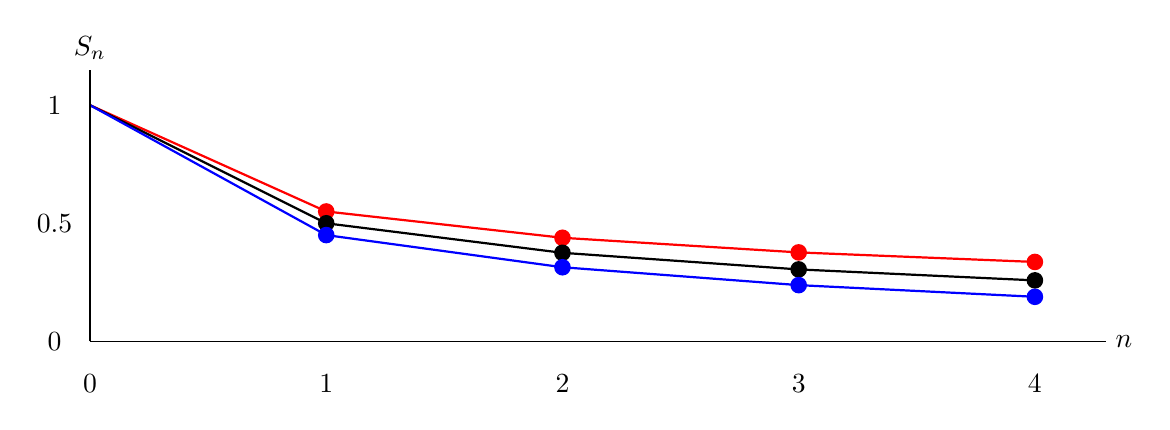
\begin{tikzpicture}[scale = 3]
    % Scatter plot points
    \foreach \x/\y/\color in {1/0.55/red, 2/0.4386250/red, 3/0.3766719/red, 4/0.336304/red,
                                                1/0.5/black, 2/0.375/black, 3/0.3046875/black, 4/0.25827/black,
                                                   1/0.449999/blue, 2/0.313874/blue, 3/0.2381546/blue, 4/0.188816/blue}
      \fill[color=\color] (\x, \y) circle (1pt);

    % Trajectories
    \draw[red, thick] (0, 1) -- (1, 0.55) -- (2, 0.4386250) -- (3,0.3766719) -- (4,0.336304);
    \draw[black, thick] (0, 1)--(1,0.5) --  (2,0.375) -- (3,0.304687) -- (4,0.25827);
    \draw[blue, thick] (0, 1)--(1,0.449999)  --  (2,0.313874) -- (3,0.238154) -- (4,0.18881);

    % Axis labels
    \draw[-] (0,0) -- (4.3,0) node[right] {$n$};
    \draw[-] (0,0) -- (0,1.15) node[above] {$S_n$};

    % Time points
    \foreach \x/\label in {0/0, 1/1/, 2/2/, 3/3, 4/4}
      \node at (\x, -0.18) {\label};
      
      \foreach \y/\label in {0/0, 0.5/0.5, 1/1/}
      \node at (-0.15, \y) {\label};
  \end{tikzpicture}

\end{center}



\subsection*{An initial infectious cohort of size $k$}
Now suppose that $X_0 = k$. Instead of the process beginning with a single unit, it starts out with a group; and for the sake illustration, we can assume this bunch is small to moderate in number, perhaps around $k = 10$.\par Given we assume supercritical branching, as the bacterial count increases, the population growth will naturally become more predictably exponential in nature. A large number of cohort units causing the expected dynamics to shine through, emergent from the haze of individual stochasticity.\par


And so, for or this initial colony --- maybe $k = 10$ pathogenic bacteria in a mammalian host --- what are its chances of persistence? Of going on to found a full blown infection?  \par
We can address this question by considering the probability with time that at least one descendent remains from the first colony. This is the likelihood that not every lineage has gone extinct. Given a single lineage dies out with the above described probability, ${}_1u_n$, the chance of all $k$ lineages dissapearing is $\lrb{{}_1u_n}^k$. Hence the probability of population persistence, in at least some descendant, is 
$$S^{(k)}_n = 1 - \lrb{{}_1u_n}^k.$$


\begin{figure}
\centering
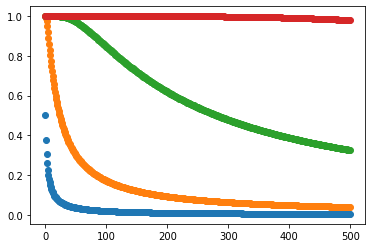
\includegraphics[width=0.6\textwidth]{chapter3/IMG_ch3/kvals.png}
\caption{Survival probability out to 500 generations with 1, 10, 100, and 1000 initial individuals. (From blue to red).  }
\label{fig1}
\end{figure}

\noindent
Figures \ref{fig1} and \ref{fig2} show the values of $S_n^{(k)}$ through 500 generation for $k$ = 11, 10, 100, and 1000. The effect seen in figure \ref{fig1}, that a greater first cohort gives improved longevity, is highly sensitive to the criticality of the process. So persistence develops quickly as $p$ approaches 0.5 from below, and it continues to improve dramatically into supercriticality. To illustrate this, figure \ref{fig2} shows the same experiment done with $p$ slightly above and below 0.5. 



\begin{figure}
\centering

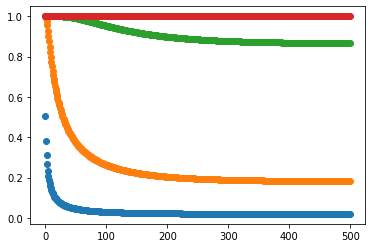
\includegraphics[width=0.45\textwidth]{chapter3/IMG_ch3/kvals505.png}
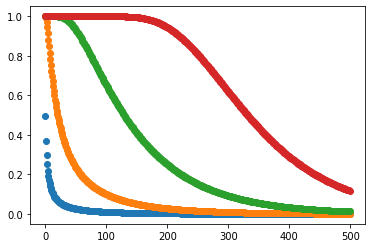
\includegraphics[width=0.45\textwidth]{chapter3/IMG_ch3/kvals495.png}
\caption{Like figure \ref{fig1} but the value of $p$ is no longer exactly critical at 0.5. On the left, it is supercritical at 0.505; for the right, 0.495. }
\label{fig2}
\end{figure}

\subsection*{Potential implications}

Firstly, it seems if nothing else a curiosity, that this observation aligns with a point made be R. Mann in a recent paper on modelling the longevity and size of phylogenetic clades. Here it was highlighted that those clades which have persisted through the ages, and are often of superior diversity, happened to have experienced an above average early rate of species origination. As far as I understand, this is an observation from the fossil record itself. Mann et al. argued that this empirical fact can be explained merely as a statistical consequence. As, if you were to run, as they did, a large number of homogeneous birth death processes, and select only those which happen to survive to some arbitrary large positive time ---  ``the present''. 





A hypothesis: It is of pathogenic advantage for an agent to ensure a high security of early initial replication, even at some cost to individual unit survival through later generations. 


\subsection{Discrete Birth-death-catastrophe --- does it have a stationary limiting distribution?}

Until the point of catastrophe, a discrete time BDC process will exhibit the same behaviour with regards to its stationary conditional limiting distribution as the basic Galton Watson model. \par
So conditioning on non-rupture, the process, when also conditioned on non extinction by death, exhibits a stationary limiting distribution. Does this mean that there will be a quasi-stationary distribution when conditioning on neither death nor catastrophe. In any case, we can test this with simulations.\par
But in addition, it will prove helpful to figure out some probability of non-catastrophe with advancing generations.
\subsection*{Probability of rupture at step $n$}

If the probability that a given individual will initiate catastrophe is $k$, the we can specify the probability that none of a size $N$ cohort will do so at an iterative step. A single individual will not cause rupture with probability $1-k$, two wp $(1-k)^2$, three, $(1-k)^3$, so on and so forth... \par
Considering for now the case of only birth and catastrophe --- no death --- it can be said with certainty the census of a living population at arbitrary generation, $n$. With a single progenitor, it is simply the case that the population will double at each step prior to catastrophe. Hence, the process will come to its abrupt halt in generation $n$ with probability
$$1-(1-k)^{2^{n-1}}$$
(not every individual didn't cause catastrophe).

\subsection*{Probability of process survival}
Thinking along these lines we can define (for the no death case)  the probability that a process survives to generation $n$. Lets call it $S_n$. For generation 0, this is clearly certain ($S_0=1$). Survival to generation one simply requires that the first individual replicated, $S_1 = (1-k)$. For persistence to step 2, not only must the first unit divide, but so must each of its offspring: $$S_2 = (1-k)(1-k)^2.$$ And so a pattern can be seen. For survival to the $n$th generation, every step prior must have been passed. Hence,
$$S_n = \Pi_{i = 0}^{n-1} (1-k)^{2^i} = (1-k)^{\sum^{n-1}_{i=0}2^i}.$$

\subsection*{Death included}
The difficulty comes in defining $S_n$ when death is allowed. In this version, the size of a living population can no longer be known with certainty through the generations. The question I would now like to address, is do the probabilities some how ``shake out'' when the expected value of the process is used; is the following correct? 
$$S_n  = (1-k)^{\sum^{n-1}_{i=0}\mean{\xx_i}}.$$
I suspect it isn't. But probably worth checking. 


\subsection{Continuous time birth death --- Survival probability and QS distribution}


From Linda Allen's book, we have the probability of extinction for the simple birth death process: 
$$p_0(t) = \begin{cases}
\lrb{\frac{\mu - \mu e^{(\mu - \lambda) t }}{  \lambda  - \mu e^{(\mu - \lambda) t }}}^N, \;\; &\lambda \neq \mu\\ 
\lrb{\frac{\lambda t}{1 + \lambda t}}^N, \;\;& \lambda = \mu.
\end{cases}$$
From this, we also have the probability of process survival at time $t$:
$$S^{(N)}(t) = 1 - p_0(t)$$

\subsection*{Limiting mean conditioned on non-extinction}
The simple birth-death model has a stationary mean when $\mu < \lambda$. We can demonstrate this simply in the following way. The conditional mean can be obtained via,
\begin{equation}
\label{condit}
\mean{\xt | \xt > 0} = \frac{\mean{\xt} }{S^{(N)}(t)}.
\end{equation}
And the late time limit of this can be evaluated using L'hopital's rule. When $\mu < \lambda$, 
$$\lim_{t\to\infty}\mean{\xt | \xt > 0}  = \frac{\mu}{\mu - \lambda} = \frac{1}{1 - \frac{\lambda}{\mu}}$$

\subsection*{More simply}

Taking $N=1$, when $\lambda < \mu$: 
$$\mean{\xt } = \ee^{(\lambda - \mu)t}$$
and,
\begin{align*}
S(t) &= 1 - \lrb{\frac{\mu - \mu \ee^{(\mu - \lambda)t}}{\lambda - \mu \ee^{(\mu-\lambda)t}}} \\
&= \frac{\lambda - \mu}{\lambda - \mu \ee^{(\mu - \lambda)t}}.
\end{align*}
So given (\ref{condit}),
$$\mean{\xt | \xt > 0} = \frac{\lambda\ee^{(\lambda-\mu)t} - \mu}{\lambda - \mu}.$$
In the case considered, $\lambda > \mu$, the limiting conditional mean becomes a constant:
$$\lim_{t\to\infty}\mean{\xt | \xt > 0}  = \frac{\mu}{\mu - \lambda}  \lrb{ = \frac{1}{A}}$$.
This may be represented as
$$\frac{1}{A} = \frac{1}{1 - \frac{\lambda}{\mu}};$$
and writing in terms of replication probability, $p = \lambda/(\lambda + \mu)$,
$$\frac{1}{A} = \frac{1-p}{1-2p};$$
inverse of the quasi-stationary mean,
$$A = \frac{1-2p}{1-p}.$$


\begin{center}
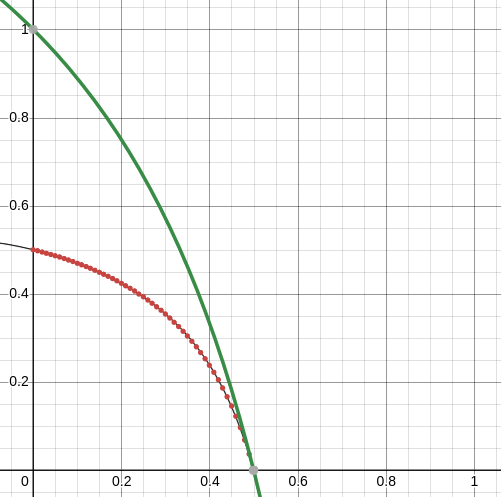
\includegraphics[width=0.45\textwidth]{chapter3/IMG_ch3/dtctA.png}
\end{center}

\noindent
In the figure above, the green line is $A$ as defined above. The red dots represent precise numerically obtained values of the analogous measure in the discrete time Galton Watson process; the black line is a closely matching formula found computationally \cite{cohen2024physics} \cite{stanley2002evolving}.\par
The obvious question which comes to mind is: why does the curve start at 1 in continuous time and 0.5 in discrete time. Merely dividing the ``green'' formula by 2 doesn't cause an overlap.





























%%%%%%%%%%%%%%%%%%%%%%%%%%%%%%%%%%%%%%%%%%%%%%%%%%%%%%%%%%%%%%%%%%%%%%%%%%%%%%%%%%%%%%%%%%%%%%%%%%%%%%%%%% MOC





\section{Method of characteristics}




In previous work, we have been successful in describing birth-death dynamics of pathogenic particles inside a host cell which can rupture. In future, we wish to extend this understanding to cases with multiple host cells sharing a medium. Setting up a model with more than one host requires consideration of what happens when the first one ruptures. The shared medium suddenly gains a potentially large cohort of pathogenic particles, available for subsequent absorption by remaining hosts. We have begun to develop the analysis under the assumption of what may be called ``immediate transfer'' --- the whole pathogenic contents of a rupturing cell being relocated to the intracellular environment of another host. This is quite a hard assumption. Another, perhaps more realistic restriction might be to incorporate an ``absorption period'': following a host cell rupture, absorption events relocate the pathogenic cohort between remaining hosts. Then, only when every pathogen has been taken in, do birth death and rupture continue. 

Working towards an understanding of such ``absorption models'', we can begin by considering processes where a pathogenic cohort infiltrate only a single host cell. 

\subsection{Only absorption} 
Perhaps the most simple case for an absorption process is that of a single host cell, able to take-in pathogenic particles, but in which no subsequent dynamics take place --- without any birth, or death of pathogen within the host. 

We can introduce the variables $\xt$ \& $\yt$ to represent the number of pathogenic particles within, and outside of the host cell respectively. The same labelling will be used in later versions of the single-host model. In all cases, events will be assumed to be stochastic, happening between exponentially distributed inter-event times. This property arises from the assumption that event-rates are time-independent. It then follows that our continuous-time stochastic process, $\{(\xt, \yt) : t\in[0,\infty\}$, conforms to the memoryless Markov property.

With only absorption to consider, the model can be specified by the following probabilities --- outcome-likelihoods over an infinitesimal duration, $\Delta t$ (taken in the limit to 0).
%\begin{equation}
  % \begin{split}
  %   \pr{\Delta\xx= 1,\;\Delta\yy = -1 \;|\; \yt = j} = j \alpha \Delta t\\
 %    \pr{\Delta\xx= 0,\;\Delta\yy = 0 \;|\; \yt = j} = 1 -  j \alpha \Delta t
 %  \end{split}
%\label{probSpec1}
%\end{equation} 
\begin{align*}
     \pr{\Delta\xx= 1,\;\Delta\yy = -1 \;|\; \yt = j} &= j \alpha \Delta t,  &&\text{(absorption)}\\
     \pr{\Delta\xx= 0,\;\Delta\yy = 0 \;|\; \yt = j} &= 1 -  j \alpha \Delta t,  &&\text{(no event)}
\end{align*} 


\noindent
where $\Delta \xx = \xx_{t+\Delta t} - \xt$ (same for $\yy$). Notice the multiplication by $j$, the number of extracellular particles --- each unit subjected to the same probability, $\alpha \Delta t$, of being taken up. 

The model's initial condition will be specified: $\xx_0 = 0$, $\yy_0 = N$. A starter population of census $N$ occupying the extracellular medium. 

Defining state probabilities, $p_{i,j}(t) = \pr{\xt = i,\; \yt = j}$, we can write down the forward Kolmogorov equations: 
\begin{equation}
\label{F1}
\ddt{\p} = \alpha(j + 1) p_{i-1,j+1} - \alpha j \p.
\end{equation}

\noindent
Then, with the probability generating function defined,
\begin{equation}
\label{pgfDef}
G(x,y,t) = \sum_i\sum_j \pt x^iy^j 
\end{equation}

\noindent
$\left(=\mathbb{E}\left[x^{\xt}y^{\yt}\right]\right)$, we can go on to derive a PDE for $G(x,y,t)$ in the following way. 

Firstly, multiply each equation in (\ref{F1}) by $x^iy^j $,
\begin{equation*}
%\label{pdeDerev1}
\pddt{\p x^iy^j} = \alpha(j + 1) p_{i-1,j+1}x^iy^j - \alpha j \p x^iy^j.
\end{equation*}

\noindent
Then sum over $i$ and $j$ for non-zero $\pt$,
\begin{equation}
\label{pdeDere2}
\sum_{i = 0}^N\sum_{j=0}^N\pddt{\p x^iy^j} = \alpha\sum_{i = 1}^{N+1}\sum_{j=-1}^{N-1}(j + 1) p_{i-1,j+1}x^iy^j - \alpha \sum_{i = 0}^N\sum_{j=0}^Nj \p x^iy^j.
\end{equation}

\noindent
(Note, for any $i, j > N$, and when $i+j \neq N$, $\pt = 0$ $\forall t$. This is because pathogenic particles in this model are neither created nor destroyed.)

Rearranging (\ref{pdeDere2}), we find 
\begin{equation*}
\label{pdeDerev2}
\sum_{i = 0}^N\sum_{j=0}^N\pddt{\p x^iy^j} = \alpha\left(x\sum_{i = 0}^N\sum_{j=0}^N j p_{i,j}x^{i}y^{j-1} -  y\sum_{i = 0}^N\sum_{j=0}^Nj \p x^iy^{j-1} \right),
\end{equation*}

\noindent
which can be written in terms of the following partial derivatives,
\begin{equation*}
\label{pdeDerev2}
\sum_{i = 0}^N\sum_{j=0}^N\pddt{\p x^iy^j} = \alpha\left(x - y\right)\sum_{i = 0}^N\sum_{j=0}^N \pdd{\p x^iy^j}{y}.
\end{equation*}

\noindent
Notice, with (\ref{pgfDef}), 
\begin{equation}
\label{PDE1}
\pddt{G(x,y,t)} = \alpha\left(x - y\right) \pdd{G(x,y,t)}{y};
\end{equation}

\noindent
the chosen initial condition corresponding to $G(x,y,0) = y^N$.
 
This first-order linear initial value problem, it turns out, proves quite difficult to solve. The method of characteristics, though practicable by definition on equations of three variables, has so far lead only to mystification.

But, as it happens, we can obtain its solution via other means. 

\subsubsection*{Benefits of the independence property}
$G(x,y,t)$, as referred to above was specific to the initial condition, $\xx_0 = 0$, $\yy_0 = N$. We may further specify the probability generating function,
\begin{equation*}
G_n(x,y,t) = \sum_i\sum_j \pr{\xt = i,\;\yt=j \;|\;\xx_0 = 0,\;\yy_0=n } x^i y^j.
\end{equation*}
In such a process of just absorption, each of the $N$ pathogenic particles will get taken up by the host cell one by one. If we were to focus our attention on a single particle of this cohort, the behaviour observed would not depend on the movements of it's neighbours. Due this property of independence, our variables $\xt$ \& $\yt$ can be thought of as the sum of $N$ sub-variables, $\xt^{(k)}$ \& $\yt^{(k)}$, each pertaining only to the movements of a single pathogenic unit: 
\begin{align*}
\xt = \xt^{(1)} + \xt^{(2)} + \dots + \xt^{(n)}\\
\yt = \yt^{(1)} + \yt^{(2)} + \dots + \yt^{(n)}
\end{align*}
This observation allows us to prove that 
\begin{equation}
\label{indRelPGF}
G_n(x,y,t) = \lrb{G_1(x,y,t)}^n:
\end{equation}
\begin{align*}
G_n(x,y,t) &= \ex{x^{\sum_{k=1}^n \xt^{(k)}} y^{\sum_{k=1}^n \yt^{(k)}}}\\
&=  \ex{\prod_{k=1}^n x^{\xt^{(k)}} \prod_{k=1}^n y^{\yt^{(k)}} }\\
&=  \prod_{k=1}^n\ex{ x^{\xt^{(k)}} y^{\yt^{(k)}} }\\
&=  \prod_{k=1}^n G_1(x,y,t)\\
&= \left(G_1(x,y,t)\right)^n
\end{align*}

\noindent
Now, consider there were only one pathogenic particle to begin with; $\xx_0 = 0$, $\yy_0 = 1$. It would after some time be absorbed, and this would be the final state of the system. No other states could be reached --- quite simply: $\pt = 0$ $\forall t$ for $i+j \neq1$.\par
We can hence fully determine the state probabilities of this simple case using the forward Kolmogorov equations.
\begin{align*}
\ddt{p_{0,1}(t)} = -\alpha p_{0,1}(t) && \ddt{p_{1,0}(t)} = \alpha p_{0,1}(t) 
\end{align*}
$\implies$
\begin{align*}
p_{0,1}(t) = \ee^{-\alpha t} && p_{1,0}(t) = 1 - \ee^{-\alpha t}
\end{align*}





\begin{figure}[H]
\begin{center}
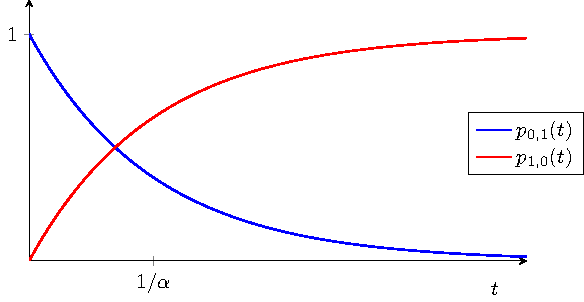
\includegraphics[width = 0.65\textwidth]{chapter3/IMG_ch3/abs1.pdf}
\end{center}
\end{figure}








\noindent
Given these represent the only two non-zero state probabilities of the single particle system, we can write-out the associated probability generating function as
\begin{align*}
G_1(x,y,t) &= p_{1,0}(t)x + p_{0,1}(t)y\\
    &=   \lrb{1-\ee^{-\alpha t} }x + \ee^{-\alpha t}y.
\end{align*}
Then, applying relation (\ref{indRelPGF}), we can define the probability generating function for this absorption-only system generally, for any initial state,
\begin{equation*}
G_n(x,y,t) = \lrb{ \lrb{1-\ee^{-\alpha t} }x + \ee^{-\alpha t}y}^n;
\end{equation*}

\noindent
noting that this does satisfy equation (\ref{PDE1}) along with its initial condition, 
$$G_n(x,y,0) = y^n.$$


%- forward kolmogorov equations

%- PDE for probability generating function 

%- note on difficulty in solving it

%- Solution allowed by independence assumption.

 
\subsection{Absorption-death}

In reality, when resident in a host-cell, pathogenic particles may be subject to death. \par
Setting-up a model as above, with $\xt$ \& $\yt$ representing the count of intracellular and extracellular pathogen, we can incorporate particle death with the following addition. 
\begin{align*}
     \pr{\Delta\xx= 1,\;\Delta\yy = -1 \;|\; \yt = j} &= j \alpha \Delta t,  &&\text{(absorption)}\\
      \pr{\Delta\xx= -1,\;\Delta\yy = 0 \;|\; \xt = i} &= i \mu \Delta t,  &&\text{(death)}\\
     \pr{\Delta\xx= 0,\;\Delta\yy = 0 \;|\; \yt = j, \xt=i} &= 1 -  \lrb{ j\alpha + i\mu}\Delta t,  &&\text{(no event)}
\label{probSpec1}
\end{align*} 

Form here, an analogous line of reasoning can be followed. A familiar difficulty is found on arrival at the first order linear PDE,
\begin{equation*}
\label{PDE2}
\pddt{G(x,y,t)} = \mu(1-x) \pdd{G(x,y,t)}{x}+\alpha\left(x - y\right) \pdd{G(x,y,t)}{y}.
\end{equation*}

\noindent
This point being reached from a similar derivation using the forward Kolmogorov equations:
\begin{equation*}
\label{FK1}
\ddt{\p} = \alpha(j + 1) p_{i-1,j+1} + \mu(i+1)p_{i+1,j} - (\alpha j + \mu i) \p.
\end{equation*}

\noindent
But as above, the solution can be constructed with a work-around employing the relation 
\begin{equation*}
G_n(x,y,t) = \lrb{G_1(x,y,t)}^n.
\end{equation*}

\noindent
As before, individual particles are independent from one another in their movements.\par
Without birth events, the maximum number of particles in the system is restricted to it's initial value. So, when considering the case of an isolated pathogenic unit, the probability generating function takes its form,
\begin{equation*}
G_1(x,y,t) = p_{0,0} + p_{1,0}x + p_{1,0}y.
\end{equation*}

\noindent
These state-probabilities can be determined as follows using the forward Kolmogorov equations. 
\begin{align*}
\ddt{p_{0,1}(t)} = -\alpha p_{0,1}(t) && \ddt{p_{1,0}(t)} = \alpha p_{0,1}(t) - \mu p_{1,0}(t)
\end{align*}
$\implies$
\begin{align*}
p_{0,1}(t) = \ee^{-\alpha t} && p_{1,0}(t) = \frac{\alpha}{\mu - \alpha} \Big(   \ee^{-\alpha t} - \ee^{-\mu t} \Big) && p_{0,0}(t) = 1 -p_{0,1}(t)  -p_{1,0}(t) 
\end{align*}





\begin{figure}[H]
\begin{center}
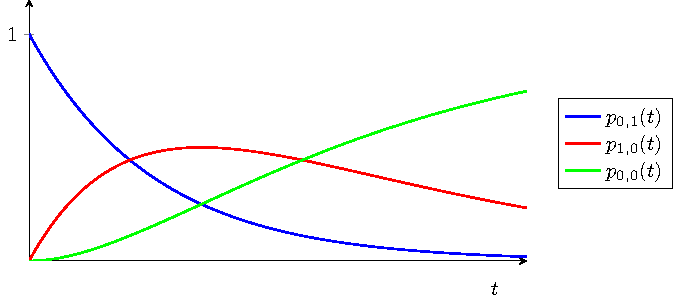
\includegraphics[width = 0.65\textwidth]{chapter3/IMG_ch3/abs2.pdf}
\end{center}
\caption{Caption}
\end{figure}
    

    


\noindent
Leading, as above, to the general probability generating function, $G_n(x,y,t)$, through relation (\ref{indRelPGF}):
\begin{equation*}
G_n(x,y,t) = \lrb{1-\frac{\mu}{\mu - \alpha}  \ee^{-\alpha t}  + \frac{\alpha}{\mu - \alpha} \ee^{-\mu t}  + \frac{\alpha}{\mu - \alpha} \Big(   \ee^{-\alpha t} - \ee^{-\mu t} \Big)x +  \ee^{-\alpha t} y}^n
\end{equation*}



%\begin{equation}
%G_1(x,y,t) = 1-\frac{\mu}{\mu - \alpha}  \ee^{-\alpha t}  + \frac{\alpha}{\mu - \alpha} \ee^{-\mu t}  + \frac{\alpha}{\mu - \alpha} \Big(   \ee^{-\alpha t} - \ee^{-\mu t} \Big)x +  \ee^{-\alpha t} y
%\end{equation}

\subsection{Method of characteristics (absorption-death)}

Before continuing to the case of absorption-birth-death where replication may occur within the host cell, let us revisit absorption-death from the point of its PDE for $G(x,y,t)$.  

\begin{equation}
\label{PDE2}
\pddt{G(x,y,t)} = \mu(1-x) \pdd{G(x,y,t)}{x}+\alpha\left(x - y\right) \pdd{G(x,y,t)}{y},
\end{equation}
with initial condition $G(x,y,0) = y^N$.

Since writing the above sections, I have been given advice by Benjamin Sharp on how to use the method of characteristics for 3 variate problems.\par
We begin by introducing a change of variables $(x,y,t) \to (s,r,\tau)$:
$$G(x,y,t) = G\big(x(s,r,\tau), y(s,r,\tau), t(s,r,\tau) \big) \equiv G(s,r,\tau)$$
The method works by seeking solutions on the characteristic surfaces of constant $s$ and $r$; $G(\tau)$. To do so, we must introduce an initial surface in the $s$, $r$, $\tau$ space:
\begin{align}
\label{ICpar}
x(s,r,0) = s && y(s,r,0) = r && t(s,r,0) = 0
\end{align}

With the probability generating a function of only one variable, $\tau$, we can write down the characteristic equations as ODEs. First, consider,
\begin{equation*}
\dda{G}{\tau} = \pddt{G} \dda{t}{\tau}  +  \pdd{G}{x}\dda{x}{\tau} + \pdd{G}{y}\dda{y}{\tau} .
\end{equation*}
Notice similarity with (\ref{PDE2}),
$$0  = -\pddt{G} + \mu(1-x)\pdd{G}{x} + \alpha (x-y)\pdd{G}{y}.$$
Comparing coefficients, we can write down the characteristic ODEs: 
\begin{align}
\dda{G}{\tau} &= 0\label{ch11}\\
\dda{t}{\tau} &= -1\label{ch12}\\
\dda{x}{\tau} &= \mu(1-x)\label{ch13}\\
\dda{y}{\tau} &= \alpha(x-y)\label{ch14}
\end{align}


\subsubsection*{(\ref{ch11})}
Solving the first characteristic equation,
$$\dda{G}{\tau} = 0$$
$$G = \phi(s,r)$$
$\phi$ constant on surfaces of constant $s$, and $r$.\par
With  (\ref{ICpar}), the initial condition on $G$ translates to $G(s,r,\tau=0) = r^N$, which informs us that $\phi(s,r) = r^N$. Hence,
\begin{equation}
\label{GrN}
G(s,r,\tau) = r^N.
\end{equation}



\subsubsection*{(\ref{ch12})}
$$\dda{t}{\tau} = -1$$
$$t = -\tau + c(s,r)$$
Using (\ref{ICpar}), we can fix the constant, $c(s,r) = 0$.
\begin{equation}
\label{minustau}
t = -\tau
\end{equation}


\subsubsection*{(\ref{ch13})}
$$\dda{x}{\tau} = \mu(1-x)$$
$$\vdots$$
$$1-x = c(s,r) \ee^{-\mu \tau}.$$
With initial condition, (\ref{ICpar}), $c(s,r) = 1-s$;
\begin{equation}
\label{sandxwithtau}
1-x = (1-s) \ee^{-\mu \tau}.
\end{equation}


\subsubsection*{(\ref{ch14})}

\begin{align*}
\dda{y}{\tau} &= \alpha(x-y)\\
\dda{y}{\tau} &= \alpha\left(1-(1-s) \ee^{-\mu \tau} -y\right)
\end{align*}
$$\vdots$$
$$y = 1 - \frac{\alpha}{\alpha-\mu}(1-s)\ee^{-\mu\tau} + c(s,r)\ee^{-\alpha\tau}.$$
Applying (\ref{ICpar}), $c(s,r) = r + \frac{\alpha}{\alpha-\mu}(1-s) -1$;
\begin{equation}
\label{ywithr1}
y = 1 - \frac{\alpha}{\alpha-\mu}(1-s)\ee^{-\mu\tau} + \lrb{r + \frac{\alpha}{\alpha-\mu}(1-s) -1}\ee^{-\alpha\tau}.
\end{equation}

\vspace{15pt}
\noindent
Finally, if we rearrange (\ref{ywithr1}) for $r$, also substituting $s(x,y,t)$ from (\ref{sandxwithtau}), and $\tau = -t$ from (\ref{minustau}), we find:
\begin{equation*}
r = 1-\frac{\mu}{\mu - \alpha}  \ee^{-\alpha t}  + \frac{\alpha}{\mu - \alpha} \ee^{-\mu t}  + \frac{\alpha}{\mu - \alpha} \Big(   \ee^{-\alpha t} - \ee^{-\mu t} \Big)x +  \ee^{-\alpha t} y
\end{equation*}
Then, with $G = r^N$ ((\ref{GrN})), this matches the solution obtained in the previous section, 
\begin{equation*}
G(x,y,t) = \lrb{1-\frac{\mu}{\mu - \alpha}  \ee^{-\alpha t}  + \frac{\alpha}{\mu - \alpha} \ee^{-\mu t}  + \frac{\alpha}{\mu - \alpha} \Big(   \ee^{-\alpha t} - \ee^{-\mu t} \Big)x +  \ee^{-\alpha t} y}^N.
\end{equation*}





\subsection{Absorption-birth-death}

Introducing replication for particles inside the host cell, we will see that though the independence property is still present, it no longer serves as a work-around in finding the probability generating function $G(x,y,t)$. This is because, given a single initial infections particle, with birth events, an infinite number of states can be reached. Hence $G_1(x,y,t)$ will be constituted by an infinite number of terms.\par

Thankfully, we are now also equipped to solve the PDEs for $G(x,y,t)$, and this is the approach we will take.\par

Setting up the model like in previous cases, $\xt$ \& $\yt$ represent the counts of intracellular and extracellular pathogenic particles. Birth events are added to the transition rates as follows.

\begin{align*}
     \pr{\Delta\xx= 1,\;\Delta\yy = -1 \;|\; \yt = j} &= j \alpha \Delta t,  &&\text{(absorption)}\\
     \pr{\Delta\xx= 1,\;\Delta\yy = 0 \;|\; \xt = i} &= i \beta \Delta t,  &&\text{(birth)}\\
      \pr{\Delta\xx= -1,\;\Delta\yy = 0 \;|\; \xt = i} &= i \mu \Delta t,  &&\text{(death)}\\
     \pr{\Delta\xx= 0,\;\Delta\yy = 0 \;|\; \yt = j, \xt=i} &= 1 -  \lrb{ j\alpha + i\mu + i\beta}\Delta t,  &&\text{(no event)}
\label{probSpec1}
\end{align*} 

The forward Kolmogorov equation is written as such.
\begin{equation*}
\label{FK3}
\pddt{\p } = \alpha(j + 1) p_{i-1,j+1} + \mu(i+1)p_{i+1,j}  +  \beta(i-1)p_{i-1,j}    -  (\alpha j + \mu i+\beta i) \p 
\end{equation*}

From here, again, with reasoning seen above, we can derive the associated PDE for $G(x,y,t)$.

\begin{equation}
\pddt{G} = \lrb{\mu - (\mu+ \beta)x + \beta x^2}\pdd{G}{x} + \alpha(x-y)\pdd{G}{y}
\end{equation}

To solve this by the method of characteristics, as above we re-parametrize $(x,y,t)$ to $(s,r,\tau)$, then seek solutions on characteristic surfaces of constant $s$ and $r$. Doing so brings us to the characteristic ODEs: 
\begin{align}
\dda{G}{\tau} &= 0\label{ch21}\\
\dda{t}{\tau} &= -1\label{ch22}\\
\dda{x}{\tau} &= \mu-(\mu+\beta)x + \beta x^2\label{ch23}\\
\dda{y}{\tau} &= \alpha(x-y)\label{ch24}
\end{align}
Applying the same initial conditions on $(s,r,\tau)$ as above in (\ref{ICpar}), we can solve these equations as follows.

\subsubsection*{(\ref{ch21}) \& (\ref{ch22})}
Like in the previous section the first two characteristic equations yield: 
$$G(s,r,\tau) = \phi(s,r),$$
and ultimately,
\begin{equation}
\label{gngngn}
G(s,r,\tau) = r^N.
\end{equation}
Then,
$$t = -\tau.$$   


\subsubsection*{(\ref{ch23})}
This equation looks remarkably like Jonty's equation for $S$, the survival probability. 
$$\dda{x}{\tau} = \beta\lrb{x-x_+}\lrb{x-x_-}$$
with,
$$x_{\pm} = \frac{\mu + \beta}{2\beta} \pm \sqrt{\lrb{\frac{\mu + \beta}{2\beta}}^2 - \frac{\mu}{\beta}}.$$
The main difference in its solution with Jonty's equation comes with an $s$ when fixing the constant of integration:
\begin{equation}
x(\tau) = \frac{x_+(s-x_-) - x_-(s-x_+)\ee^{\beta(x_+-x_-)\tau}}{(s-x_-) - (s-x_+)\ee^{\beta(x_+-x_-) \tau}}
\label{xabd}
\end{equation}


\subsubsection*{(\ref{ch24})}
The last characteristic equations is
$$\dda{y}{\tau} = \alpha(x-y).$$
To solve this we will need to substitute $x$ as found above, (\ref{xabd}). With an integrating factor, the equation becomes,
$$\dda{}{\tau}\lrb{\ee^{\alpha\tau} y} = \alpha \ee^{\alpha\tau} x(\tau).$$
Integrating with respect to $\tau$,
$$\ee^{\alpha\tau }y = \alpha\int \ee^{\alpha\tau} \frac{x_+(s-x_-) - x_-(s-x_+)\ee^{\beta(x_+-x_-)\tau}}{(s-x_-) - (s-x_+)\ee^{\beta(x_+-x_-) \tau}} \dd\tau.$$ 
Then splitting the numerator, 
\begin{align}
\label{bigdoubleints}
\ee^{\alpha\tau }y &=  \alpha x_+(s-x_-) \int \frac{ \ee^{\alpha \tau} } {(s-x_-) - (s-x_+)\ee^{\beta(x_+-x_-) \tau}}\dd\tau \notag \\ 
&-\alpha x_-(s-x_+)\int\frac{\ee^{\left[ \alpha + \beta(x_+-x_-) \right]\tau}}{(s-x_-) - (s-x_+)\ee^{\beta(x_+-x_-) \tau}}\dd\tau.
\end{align}

\noindent
Each of these integrals can be written in the form,
\begin{equation*}
I(\tau) = \int\frac{\ee^{h\tau}}{p+q\ee^{k\tau}}\dd\tau.
\end{equation*}
where $h$, $k$, $p$, $q$ are all constants. For example, in the first integral, $h = \alpha$, $k = \beta(x_+ - x_-)$, $p = (s-x_-)$, and $q = -(s-x_+)$. As it happens, we can solve this integral with: 
\begin{equation}
\label{hypIden}
I(\tau) = \frac{\ee^{h\tau}}{ph} {}_2F_1\lrb{1,\frac{h}{k};\frac{h}{k}+1; -\frac{q}{p}\ee^{k\tau}} + \text{const}.
\end{equation}
${}_2F_1(a,b;c;z)$ being the hypergeometric function, defined,
\begin{equation*}
{}_2F_1(a,b;c;z) =\sum^\infty_{n=0}\frac{(a)_n(b)_n}{(c)_n}\frac{z^n}{n!},
\end{equation*}
and $(p)_n$ is the (rising) Pochhammer  symbol:
$$(p)_n = \begin{cases} 1 &n=1\\
p(p+1)\cdots(p+n-1) &n>1
\end{cases}
$$
See appendix \ref{appxa} for a detailed derivation of (\ref{hypIden}).\par
Picking up again at (\ref{bigdoubleints}), the integrals are specified by (\ref{hypIden}):\\
(using $b_1 = \beta(x_+ - x_-)$ for convenience)
\begin{equation*}
\int \frac{ \ee^{\alpha \tau} } {(s-x_-) - (s-x_+)\ee^{b_1 \tau}}\dd\tau =  \frac{\ee^{\alpha\tau}}{\alpha(s-x_-)} {}_2F_1\lrb{1,\frac{\alpha}{b_1 };\frac{\alpha}{b_1 }+1; \frac{(s-x_+)}{(s-x_-)}\ee^{b_1  \tau}},
\end{equation*}
and
\begin{equation*}
\int\frac{\ee^{\left[ \alpha +b_1\right]\tau}}{(s-x_-) - (s-x_+)\ee^{b_1 \tau}}\dd\tau =   \frac{\ee^{(\alpha+b_1 )\tau}}{(\alpha+b_1 )(s-x_-)} {}_2F_1\lrb{1,\frac{\alpha + b_1 }{b_1 };\frac{\alpha + b_1 }{b_1 }+1; \frac{(s-x_+)}{(s-x_-)}\ee^{b_1  \tau}}.
\end{equation*}
Referring to these formulas as $I_1(s,r,\tau)$ and $I_2(s,r,\tau)$ respectively, and substituting into (\ref{bigdoubleints}): 
\begin{equation}
\label{eywithconst}
\ee^{\alpha\tau }y = \alpha x_+(s-x_-)I_1(s,r,\tau) - \alpha x_- (s-x_+) I_2(s,r,\tau) + \text{const}.
\end{equation}
From her, our initial condition, $y(s,r,0) = r$, fixes the constant ---
$$\text{const} = r -  \alpha x_+(s-x_-)I_1(s,r,0) + \alpha x_- (s-x_+) I_2(s,r,0).$$ 
Then, with a rearrangement of (\ref{eywithconst}), 
\begin{equation*}
r = \ee^{\alpha\tau }y - \alpha x_+(s-x_-)I_1(s,r,\tau) + \alpha x_- (s-x_+) I_2(s,r,\tau) +  \alpha x_+(s-x_-)I_1(s,r,0) - \alpha x_- (s-x_+). I_2(s,r,0)
\end{equation*}
With $I_1$, $I_2$ written explicitly,
\begin{align*}
r &= \\
 &\ee^{\alpha\tau }y\\ 
 &- \lrb{x_+ \ee^{\alpha\tau}}{}_2 F_1 \lrb{1,\frac{\alpha}{b_1 };\frac{\alpha}{b_1 }+1; \frac{(s-x_+)}{(s-x_-)}\ee^{b_1  \tau}}\\
&+\lrb{\frac{\alpha  }{\alpha + b_1}x_-\ee^{(\alpha + b_1)\tau}}{}_2F_1\lrb{1,\frac{\alpha + b_1 }{b_1 };\frac{\alpha + b_1 }{b_1 }+1; \frac{(s-x_+)}{(s-x_-)}\ee^{b_1  \tau}}\\
&+ \lrb{x_+}{}_2 F_1 \lrb{1,\frac{\alpha}{b_1 };\frac{\alpha}{b_1 }+1; \frac{(s-x_+)}{(s-x_-)}}\\
&- \lrb{\frac{\alpha  }{\alpha + b_1}x_-}{}_2F_1\lrb{1,\frac{\alpha + b_1 }{b_1 };\frac{\alpha + b_1 }{b_1 }+1; \frac{(s-x_+)}{(s-x_-)}}
\end{align*}

\noindent
From (\ref{xabd}), we have the relation,
$$\lrb{\frac{s-x_+}{s-x_-}} = \lrb{\frac{x-x_+}{x-x_-}}\ee^{b_1\tau},$$
which, applied to  the above, along with the switch, $\tau = -t$, yields 

\begin{align*}
r &= \\
 &\ee^{-\alpha t }y\\ 
 &- \lrb{x_+ \ee^{-\alpha t}}{}_2 F_1 \lrb{1,\frac{\alpha}{b_1 };\frac{\alpha}{b_1 }+1; \frac{(x-x_+)}{(x-x_-)}}\\
&+\lrb{\frac{\alpha  }{\alpha + b_1}x_-\ee^{-(\alpha + b_1)t}}{}_2F_1\lrb{1,\frac{\alpha + b_1 }{b_1 };\frac{\alpha + b_1 }{b_1 }+1; \frac{(x-x_+)}{(x-x_-)}}\\
&+ \lrb{x_+}{}_2 F_1 \lrb{1,\frac{\alpha}{b_1 };\frac{\alpha}{b_1 }+1; \frac{(x-x_+)}{(x-x_-)}\ee^{b_1  t}}\\
&- \lrb{\frac{\alpha  }{\alpha + b_1}x_-}{}_2F_1\lrb{1,\frac{\alpha + b_1 }{b_1 };\frac{\alpha + b_1 }{b_1 }+1; \frac{(x-x_+)}{(x-x_-)}\ee^{b_1  t}}
\end{align*}

\noindent
Finally, with (\ref{gngngn}),
\begin{align*}
G(x,y,t) &=\\
 &\Bigg[\ee^{-\alpha t }y\\ 
 &- \lrb{x_+ \ee^{-\alpha t}}{}_2 F_1 \lrb{1,\frac{\alpha}{b_1 };\frac{\alpha}{b_1 }+1; \frac{(x-x_+)}{(x-x_-)}}\\
&+\lrb{\frac{\alpha  }{\alpha + b_1}x_-\ee^{-(\alpha + b_1)t}}{}_2F_1\lrb{1,\frac{\alpha + b_1 }{b_1 };\frac{\alpha + b_1 }{b_1 }+1; \frac{(x-x_+)}{(x-x_-)}}\\
&+ \lrb{x_+}{}_2 F_1 \lrb{1,\frac{\alpha}{b_1 };\frac{\alpha}{b_1 }+1; \frac{(x-x_+)}{(x-x_-)}\ee^{b_1  t}}\\
&- \lrb{\frac{\alpha  }{\alpha + b_1}x_-}{}_2F_1\lrb{1,\frac{\alpha + b_1 }{b_1 };\frac{\alpha + b_1 }{b_1 }+1; \frac{(x-x_+)}{(x-x_-)}\ee^{b_1  t}}\Bigg]^N
\end{align*}


The following fact offers only some consolation from the unwieldiness of this formula.

$${}_2F_1\lrb{1,\delta;\delta+1;z} = \sum^\infty_{n=0}\frac{(1)_n(\delta)_n}{(\delta+1)_n}\frac{z^n}{n!} = \sum^\infty_{n=0}\frac{\delta}{\delta+n}{z^n}. $$

True, because along with $(1)_n = n!$, it can also be seen that 

$$\frac{(\delta)_n}{(\delta+1)n} = \frac{\delta\cancel{(\delta+1)}\cdots\cancel{(\delta + n-2)}\cancel{(\delta + n-1)}}{\cancel{(\delta+1)}\cancel{(\delta+2)}\cdots\cancel{(\delta + n-1)}(\delta + n)} = \frac{\delta}{\delta+n}.$$








\subsection*{Appendix}

\subsection{Deriving the integral result (\ref{hypIden})}\label{appxa}
To demonstrate result, 
$$\int\frac{\ee^{h\tau}}{p+q\ee^{k\tau}}\dd\tau= \frac{\ee^{h\tau}}{ph} {}_2F_1\lrb{1,\frac{h}{k};\frac{h}{k}+1; -\frac{q}{p}\ee^{k\tau}} + \text{const},$$
we will use the hypergeometric integral identity:

\begin{equation}
\label{idenHyp}
{}_2F_1(a,b;c;z) = \frac{\Gamma(c)}{\Gamma(b)\Gamma(c-b)}\int^1_0 u^{b-1}(1-u)^{c-b-1}(1-zu)^{-a} \dd u
\end{equation}
($\Gamma(x)$, being the standard gamma function). 

Taking the integral,
$$I(\tau) = \int\frac{\ee^{h\tau}}{p+q\ee^{k\tau}}\dd\tau.$$
Begin by applying the substitution, $v = \ee^{k\tau}$; with $\dd\tau = k^{-1}v^{-1} \dd v$.
\begin{align*}
I(v(\tau)) &= \frac{1}{k}\int\frac{v^{\frac{h}{k}}}{p+qv}v^{-1}\dd v\\
\notag\\
&= \frac{1}{pk}\int\frac{v^{\frac{h}{k}-1}}{1+\frac{q}{p}v}\dd v.
\end{align*}
Re-writing this as a definite integral from 0 to $v$ using a dummy variable, $s$,
$$I(v(\tau)) = \frac{1}{pk}\int^v_0\frac{s^{\frac{h}{k}-1}}{1+\frac{q}{p}s}\dd s.$$
Then, changing variables again with $s = vu$ (as $v$ is constant with regards to the definite integral, $\dd s = v\dd u$).
\begin{align}
I(v(\tau)) &= \frac{1}{pk}\int^1_0\frac{(vu)^{\frac{h}{k}-1}}{1+\frac{q}{p}vu} v \dd u\notag\\
\notag\\
&= \frac{v^{\frac{h}{k}}}{pk}\int^1_0\frac{u^{\frac{h}{k}-1}}{1+\frac{q}{p}vu}  \dd u.\label{backat}
\end{align}

\noindent
We see, this integrand lines up with that of the identity, (\ref{idenHyp});
\begin{equation*}
\int^1_0u^{\frac{h}{k}-1}(1-u)^0 \left(1-\left(-\frac{q}{p}v\right) u\right)^{-1} \dd u= \int^1_0 u^{b-1}(1-u)^{c-b-1}(1-zu)^{-a} \dd u.
\end{equation*}

\noindent
Notice, $b = \frac{h}{k}$, $c = \frac{h}{k}+1$,  $a = 1$,  and $z = -\frac{q}{p}v$. Hence,
\begin{align*}
\int^1_0\frac{u^{\frac{h}{k}-1}}{1+\frac{q}{p}vu}  \dd u &= \frac{\Gamma\left(\frac{h}{k}\right) \Gamma\lrb{1}}{\Gamma\lrb{\frac{h}{k} +1}} {}_2F_1\lrb{1,\frac{h}{k};\frac{h}{k}+1; -\frac{q}{p}v}\\
\notag\\
&= \frac{k}{h} {}_2F_1\lrb{1,\frac{h}{k};\frac{h}{k}+1; -\frac{q}{p}v},
\end{align*}
and, with (\ref{backat}),
\begin{equation*}
I(v(\tau)) = \frac{v^{\frac{h}{k}}}{ph}{}_2F_1\lrb{1,\frac{h}{k};\frac{h}{k}+1; -\frac{q}{p}v}.
\end{equation*}
Finally,
$$I(\tau) = \frac{\ee^{h\tau}}{ph}{}_2F_1\lrb{1,\frac{h}{k};\frac{h}{k}+1; -\frac{q}{p}\ee^{k\tau}}\hspace{17pt} (+ \text{const}).$$


\subsection{Extracting coefficients from the PGF -- a special case}

For a probability generating function defined not in terms of a series sum --- for example, 
\begin{equation}
\label{examplePgf}
G(t;x,y) =  \lrb{\lrb{1-\ee^{-\alpha t}}x + \ee^{-\alpha t}y}^n
\end{equation}
--- it is possible to make a conversion to its equivalent of the form,
\begin{equation}
\label{series1}
G(t;x,y) = \sum^{\infty}_{i=0}\sum^{\infty}_{j=0} p_{i,j}(t)x^iy^j.
\end{equation}
Thus extracting the time-dependent state probabilities, $p_{i,j}(t)$. It is required only that the formula $G(t;x,y)$ can be partially differentiated continuously in $x$ and $y$.\par
Here's why: A bivariate generalisation of the Maclaurin expansion can be written,
$$f(x,y)\approx Q(x,y) = \sum^{\infty}_{k=0} \lrb{\frac{1}{k!} \sum^{\infty}_{r=0}{k \choose r} \partial_x^r \partial_y^{k-r}f\bigg |_{(0,0)} x^r y^{k-r} }. $$
So, the coefficients of (\ref{series1}) can be generated via,
\begin{equation}
\label{stateProb}
p_{i,j}(t) = \lrb{i!j!}^{-1} \partial_x^i \partial_y^{j}f\big |_{(0,0)}.
\end{equation}

\subsection*{A special case}


For a probability generating function of the form,
$$G(t;x,y) = \lrb{c(t) + f(t) x + g(t) y}^n,$$
its partial derivatives in $x$ and $y$ can be obtained through
$$\partial_x^a\partial_y^b G = \lrbs{nf(t)}^a\lrbs{ng(t)}^bG.$$
With these derivatives, the state probabilities can be extracted using (\ref{stateProb}):
\begin{equation}
\label{stateProbSpec}
p_{i,j}(t) = \lrb{i!j!}^{-1} \lrbs{nf(t)}^i\lrbs{ng(t)}^jG(0,0).
\end{equation}
In this special case, $G(0,0) = (c(t))^n;$
\begin{equation}
\label{stateProbSpec2}
p_{i,j}(t) = \lrb{i!j!}^{-1} \lrbs{nf(t)}^i\lrbs{ng(t)}^j\lrbs{c(t)}^n.
\end{equation}
\subsection*{Applied to PGFs from absorption only and absorption-death }
Taking (\ref{examplePgf}), for example:
$$p_{i,j}(t) = \frac{n^{i+j}}{\lrb{i!j!}} \lrbs{1-\ee^{-\alpha t}}^i\lrbs{\ee^{-\alpha t}}^j.$$
The same can be done for 
$$G(t;x,y) = \lrb{1-\frac{\mu}{\mu - \alpha}  \ee^{-\alpha t}  + \frac{\alpha}{\mu - \alpha} \ee^{-\mu t}  + \frac{\alpha}{\mu - \alpha} \Big(   \ee^{-\alpha t} - \ee^{-\mu t} \Big)x +  \ee^{-\alpha t} y}^n$$
from the absorption-death case:
$$p_{i,j}(t) = \frac{n^{i+j}}{\lrb{i!j!}} \lrbs{\frac{\alpha}{\mu - \alpha} \Big(   \ee^{-\alpha t} - \ee^{-\mu t} \Big)}^i\lrbs{\ee^{-\alpha t}}^j\lrbs{1-\frac{\mu}{\mu - \alpha}  \ee^{-\alpha t} + \frac{\alpha}{\mu - \alpha} \ee^{-\mu t}}^n.$$





















